\documentclass{beamer}
\usetheme{CambridgeUS}

%\usepackage[utf8]{inputenc}
\usepackage[scaled=0.92]{helvet}
\usepackage{tikz}
\usepackage{amsmath, amssymb}
\usepackage{pgf}
\usetikzlibrary{calc}
\usetikzlibrary{decorations.pathreplacing}
\usetikzlibrary{positioning}
\usetikzlibrary{intersections} 
\usepackage{textcomp}
\usepackage{graphicx}
\usepackage{array}
\usepackage{booktabs}
\usepackage{epstopdf}
\usepackage{color}
\usepackage{alltt}
\usepackage{hyperref}
\usepackage{listings}
\usetikzlibrary{calc}
\usetikzlibrary{decorations.pathreplacing}
\usetikzlibrary{arrows, shapes, shadows, positioning}
\usepackage{caption}
\usepackage{subcaption}
%\usepackage{courier}
%\usepackage{default}

\title[]{LDPC Codes, Construction and Applications}
\author[Manu T S]{Manu T S \\ {\footnotesize Advisor : Prof. Sibi Raj B Pillai}}
\institute[IITB]{IIT Bombay}

\begin{document}

  % Slide 1 starts
  \frame{\titlepage}
  % Slide 1 ends

    \begin{frame}{What is an LDPC Code}
    \begin{block}{A linear error correcting code}
      All codewords should satisfy
      \begin{equation}
       \mathbf{Hx} = \mathbf{0}
      \end{equation}
      Any vector that satisfy above equation is a codeword
    \end{block}
    \begin{block}{A block code}
      If \textbf{H} is $M$ x $N$ and has rank $R$ then the code has dimension
      \begin{center}
	$K = N - R$
      \end{center}
      Block length of the code is $N$.
    \end{block}
    \begin{block}{Sparse \textbf{H}}
      Here we are dealing with binary LDPC codes, so H has few 1s rest all zeros
    \end{block}
  \end{frame}
  % Slide  ends
%   
  % Slide starts
  \begin{frame}{Tanner Graph}
    \begin{equation}
      \label{H_matrix}
      \mathbf{H} = 
      \left(
      \begin{array}{ccccccc}
      1 & 1 & 0 & 1 & 1 & 0 & 0  \\
      1 & 0 & 1 & 1 & 0 & 1 & 0  \\
      0 & 1 & 1 & 1 & 0 & 0 & 1 
      \end{array}
      \right)
    \end{equation}
    \begin{figure}
    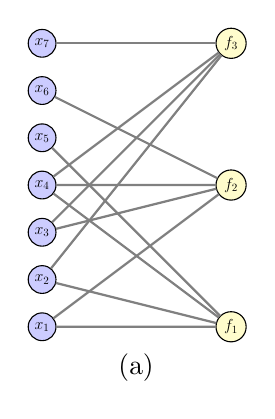
\begin{tikzpicture}[scale = 0.6, var node/.style={scale = 0.4, circle,fill=blue!20,draw,font=\sffamily\Large\bfseries}, fun node/.style={scale = 0.4, circle,fill=yellow!20,draw,font=\sffamily\Large\bfseries}]
      \node[var node] (x7) at (0, 0) {$x_7$};
      \node[var node] (x6) at (0, -1) {$x_6$};
      \node[var node] (x5) at (0, -2) {$x_5$};
      \node[var node] (x4) at (0, -3) {$x_4$};
      \node[var node] (x3) at (0, -4) {$x_3$};
      \node[var node] (x2) at (0, -5) {$x_2$};
      \node[var node] (x1) at (0, -6) {$x_1$};  
      \node[fun node] (f3) at (4, 0) {$f_3$};
      \node[fun node] (f2) at (4, -3) {$f_2$};
      \node[fun node] (f1) at (4, -6) {$f_1$};
      \draw[thick,draw=gray!100] (x1) -- node [below = 6pt] {(a)} (f1);
      \draw[thick,draw=gray!100] (x2) --  (f1);
      \draw[thick,draw=gray!100] (x4) --  (f1);
      \draw[thick,draw=gray!100] (x5) --  (f1);
      \draw[thick,draw=gray!100] (x1) --  (f2);
      \draw[thick,draw=gray!100] (x3) --  (f2);
      \draw[thick,draw=gray!100] (x4) --  (f2);
      \draw[thick,draw=gray!100] (x6) --  (f2);
      \draw[thick,draw=gray!100] (x3) --  (f3);
      \draw[thick,draw=gray!100] (x2) --  (f3);
      \draw[thick,draw=gray!100] (x4) --  (f3);
      \draw[thick,draw=gray!100] (x7) --  (f3);
    \end{tikzpicture}
    \end{figure}
  \end{frame}
  
  % Slide starts
  \begin{frame}{Degree Distribution}
    Let $\lambda$ and $\rho$ be vectors such that their $i^{th}$ component $\lambda_i$ and $\rho_i$ represent the fraction of edges
    connecting to a variable node of degree $i$ and check node of degree $i$ respectively. Thus
    \begin{equation}\nonumber
    \lambda(x) = \displaystyle \sum_i \lambda_ix^{i-1} \hspace{8pt}\text{and}\hspace{8pt} \rho(x) = \displaystyle \sum_i \rho_ix^{i-1}
    \end{equation}
    are called variable and check degree distribution polynomials respectively.
    \begin{itemize}
     \item Regular LDPC Codes
     \item Irregular LDPC Codes
     \item Ensemble LDPC($n, \lambda, \rho $)
    \end{itemize}
  \end{frame}
  % Slide ends

  \begin{frame}{Marginalization by Message Passing}
    For
    \begin{equation*}
      f(x_1,x_2,x_3,x_4,x_5,x_6) = f_1(x_1,x_2,x_3)f_2(x_1,x_4,x_6)f_3(x_4)f_4(x_4, x_5) \label{eq:fx}
    \end{equation*}
    \begin{eqnarray}
      f(x_1) 	=\sum_{x_2, x_3, x_4, x_5, x_6} f(x_1,x_2,x_3,x_4,x_5,x_6) \nonumber \\
	=\left[\sum_{x_2, x_3} f_1(x_1, x_2, x_3)\right]\left[\sum_{x_4}f_3(x_4)\left(\sum_{x_6}f_2(x_1, x_4, x_6)\right)\left(\sum_{x_5}f_4(x_4, x_5)\right)\right] \nonumber
    \end{eqnarray}
  \end{frame}
  
  \begin{frame}{Factor Graph}
      For
    \begin{equation*}
  \left[\sum_{x_2, x_3} f_1(x_1, x_2, x_3)\right]\left[\sum_{x_4}f_3(x_4)\left(\sum_{x_6}f_2(x_1, x_4, x_6)\right)\left(\sum_{x_5}f_4(x_4, x_5)\right)\right]
    \end{equation*}
   \begin{figure}[scale=0.7]
  \begin{center}
  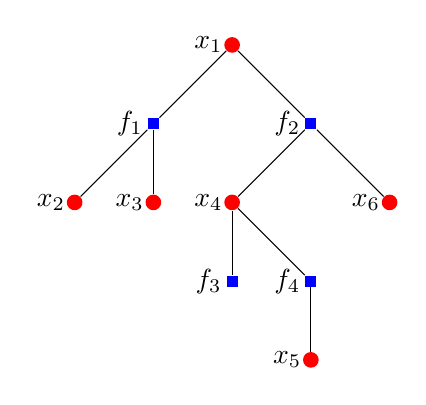
\begin{tikzpicture}[scale=1]
 \tikzstyle{cnode}=[rectangle, inner sep = 2pt, fill]
 \tikzstyle{vnode}=[circle, inner sep = 2pt, fill]
% \draw[color=red] (0,-2) node[vnode] (x2) {}; 
% \draw (-0.7, -2) node{$x_2$};
\draw [color=red](2,-2) node[vnode] (x1) {};
\draw (1.7, -2) node{$x_1$};
\draw [color=red](0,-4) node[vnode] (x2) {};
\draw (-0.3, -4) node{$x_2$};
\draw[color=red] (1,-4) node[vnode] (x3) {};
\draw (0.7, -4) node{$x_3$};
\draw[color=red] (2,-4) node[vnode] (x4) {};
\draw (1.7, -4) node{$x_4$};
\draw[color=blue] (2,-5) node[cnode] (f3) {};
\draw (1.7, -5) node{$f_3$};
\draw[color=blue] (3,-5) node[cnode] (f4) {};
\draw (2.7, -5) node{$f_4$};
\draw[color=red] (4,-4) node[vnode] (x6) {};
\draw (3.7, -4 ) node{$x_6$};
\draw[color=red] (3,-6) node[vnode] (x5) {};
\draw (2.7, -6) node{$x_5$};
\draw[color=blue] (1,-3) node[cnode] (f1) {};
\draw (0.7, -3) node{$f_1$};
\draw[color=blue] (3,-3) node[cnode] (f2) {};
\draw (2.7, -3) node{$f_2$};
\draw (x1) -- (f1);
\draw (x1) -- (f2);
\draw (f1) -- (x2);
\draw (f1) -- (x3);
\draw (f2) -- (x4);
\draw (f2) -- (x6);
\draw (x4) -- (f3);
\draw (f4) -- (x5);
\draw (x4) -- (f4);
\end{tikzpicture}
  \end{center}
  \end{figure}
  \end{frame}
  
  \begin{frame}{Message Passing Rules}
   \begin{figure}
  \begin{center}
  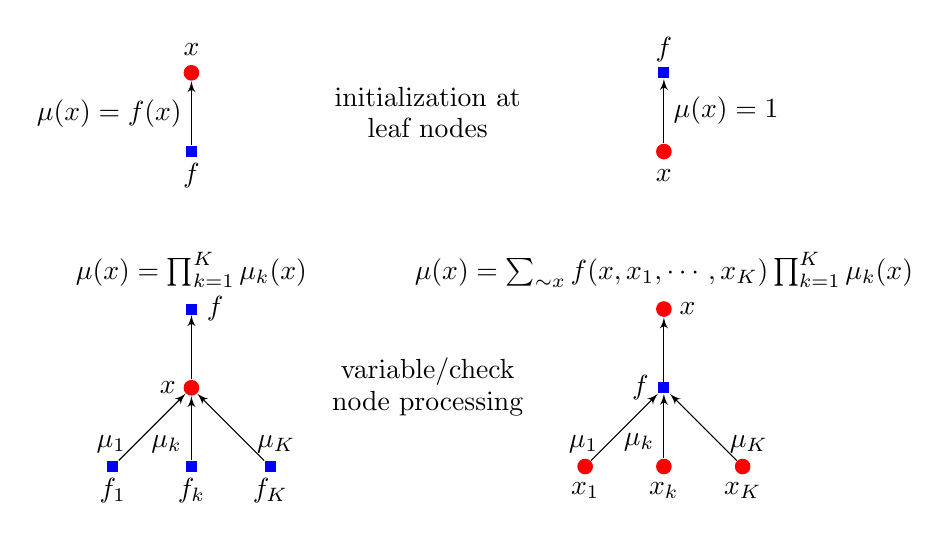
\begin{tikzpicture}[scale=1]
 \tikzstyle{cnode}=[rectangle, inner sep = 2pt, fill]
 \tikzstyle{vnode}=[circle, inner sep = 2pt, fill]
 \tikzstyle{line} = [draw, -latex']
 
 \begin{scope}
 \begin{scope}[xshift=-3cm]
    \draw[color=red] (0, 0) node[vnode] (x) {};
    \draw (0, 0.3) node{$x$};
    \draw[color=blue] (0,-1) node[cnode] (f) {};
    \draw (0, -1.3) node{$f$};
    \path [line] (f) -- node[left]{$\mu(x) = f(x)$} (x);
 \end{scope}

 \begin{scope}
  \draw (0, -0.30) node{initialization at};
  \draw (0, -0.70) node{leaf nodes};
 \end{scope}

 \begin{scope}[xshift=3cm]
    \draw[color=blue] (0, 0) node[cnode] (f) {};
    \draw (0, 0.3) node{$f$};
    \draw[color=red] (0,-1) node[vnode] (x) {};
    \draw (0, -1.3) node{$x$};
    \path [line] (x) -- node[right]{$\mu(x) = 1$} (f);  
  \end{scope}
  \end{scope}

  \begin{scope}[yshift=-3cm]
  \begin{scope}[xshift=-3cm]
 \draw[color=blue] (0, 0) node[cnode] (f) {};
 \draw (0.3, 0) node{$f$};
 \draw (0, 0.5) node{$\mu(x) = \prod_{k=1}^{K} \mu_k(x)$};
 \draw[color=red] (0,-1) node[vnode] (x) {};
 \draw (-0.3, -1) node{$x$};
 \draw[color=blue] (-1, -2) node[cnode] (f1) {};
 \draw (-1, -2.3) node{$f_1$};
 \draw[color=blue] (0, -2) node[cnode] (fk) {};
 \draw (0, -2.3) node{$f_k$};
 \draw[color=blue] (1, -2) node[cnode] (fK) {};
 \draw (1, -2.3) node{$f_K$};
 \path [line] (x) -- (f);
 \path [line] (f1) -- node[near start, left]{$\mu_1$} (x);
 \path [line] (fk) -- node[near start, left]{$\mu_k$} (x);
 \path [line] (fK) -- node[near start, right]{$\mu_K$} (x);
  \end{scope}
  
  \begin{scope}
    \draw (0, -0.80) node{variable/check};
    \draw (0, -1.20) node{node processing}; 
  \end{scope}

  \begin{scope}[xshift=3cm]
 \draw[color=red] (0, 0) node[vnode] (x) {};
 \draw (0.3, 0) node{$x$};
 \draw (0, 0.5) node{$\mu(x) = \sum_{\sim x}f(x, x_1, \cdots, x_K)\prod_{k=1}^{K} \mu_k(x)$};
 \draw[color=blue] (0,-1) node[cnode] (f) {};
 \draw (-0.3, -1) node{$f$};
 \draw[color=red] (-1, -2) node[vnode] (x1) {};
 \draw (-1, -2.3) node{$x_1$};
 \draw[color=red] (0, -2) node[vnode] (xk) {};
 \draw (0, -2.3) node{$x_k$};
 \draw[color=red] (1, -2) node[vnode] (xK) {};
 \draw (1, -2.3) node{$x_K$};
 \path [line] (f) -- (x);
 \path [line] (x1) -- node[near start, left]{$\mu_1$} (f);
 \path [line] (xk) -- node[near start, left]{$\mu_k$} (f);
 \path [line] (xK) -- node[near start, right]{$\mu_K$} (f);
  \end{scope}
  \end{scope}
  
\end{tikzpicture}
  \end{center}
  \end{figure}
  \end{frame}
  
  \begin{frame}{Message Passing Rules}
   \begin{figure}
  \begin{center}
  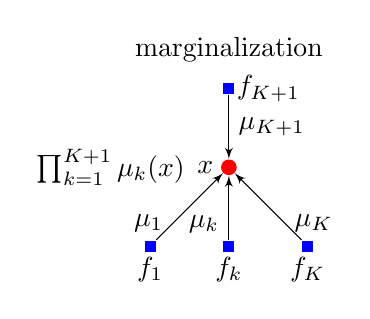
\begin{tikzpicture}[scale=1]
 \tikzstyle{cnode}=[rectangle, inner sep = 2pt, fill]
 \tikzstyle{vnode}=[circle, inner sep = 2pt, fill]
 \tikzstyle{line} = [draw, -latex']
  
 \draw[color=blue] (0, 0) node[cnode] (f) {};
 \draw (0.5, 0) node{$f_{K + 1}$};
 \draw (0, 0.5) node{marginalization};
 \draw[color=red] (0,-1) node[vnode] (x) {};
 \draw (-0.3, -1) node{$x$};
 \draw[color=blue] (-1, -2) node[cnode] (f1) {};
 \draw (-1, -2.3) node{$f_1$};
 \draw[color=blue] (0, -2) node[cnode] (fk) {};
 \draw (0, -2.3) node{$f_k$};
 \draw[color=blue] (1, -2) node[cnode] (fK) {};
 \draw (1, -2.3) node{$f_K$};
 \draw (-1.5, -1) node{$\prod_{k=1}^{K+1} \mu_k(x)$};
 \path [line] (f) -- node[right] {$\mu_{K + 1}$} (x);
 \path [line] (f1) -- node[near start, left]{$\mu_1$} (x);
 \path [line] (fk) -- node[near start, left]{$\mu_k$} (x);
 \path [line] (fK) -- node[near start, right]{$\mu_K$} (x);
  
\end{tikzpicture}
  \end{center}
  \end{figure}
  \end{frame}
  
  \begin{frame}{Message Passing Example}
   \begin{figure}
    \centering
      \begin{subfigure}{0.3\textwidth}
    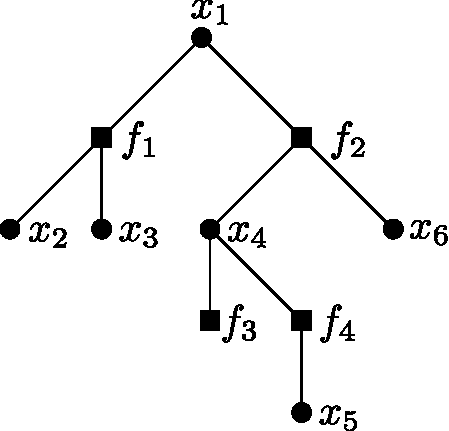
\includegraphics[scale=0.6]{factor_graph}
  \end{subfigure}
  \hspace{1.5cm}
  \begin{subfigure}{0.3\textwidth}
    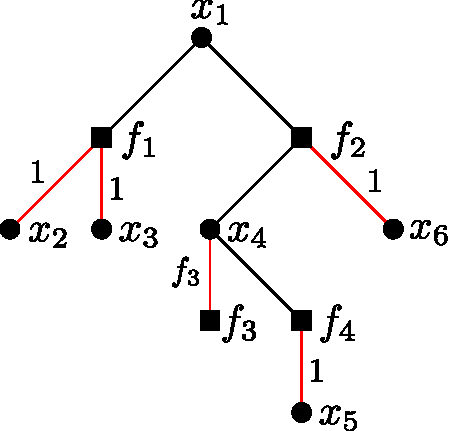
\includegraphics[scale=0.6]{factor_graph_step1}
  \end{subfigure}
   \end{figure}

  \end{frame}

    \begin{frame}{Message Passing Example}
   \begin{figure}
    \centering
  \begin{subfigure}{0.3\textwidth}
    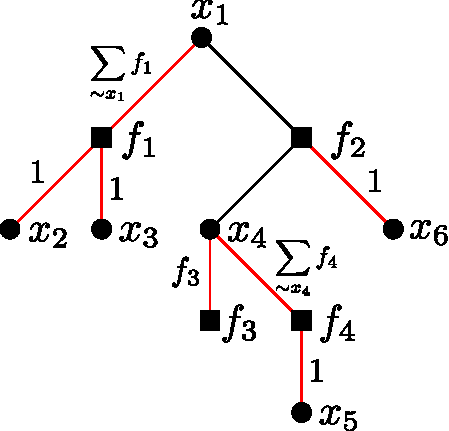
\includegraphics[scale=0.6]{factor_graph_step2}
  \end{subfigure}
  \hspace{1.5cm}
  \begin{subfigure}{0.3\textwidth}
    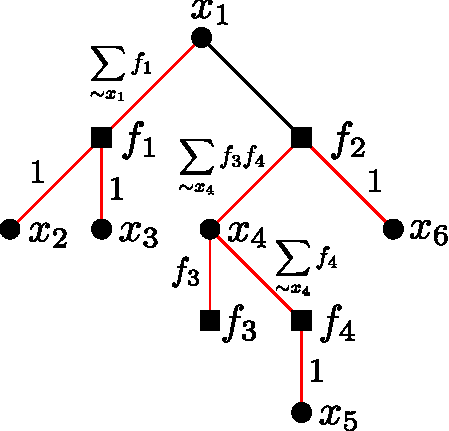
\includegraphics[scale=0.6]{factor_graph_step3}
  \end{subfigure}
   \end{figure}

  \end{frame}
  
      \begin{frame}{Message Passing Example}
   \begin{figure}
    \centering
  \begin{subfigure}{0.3\textwidth}
    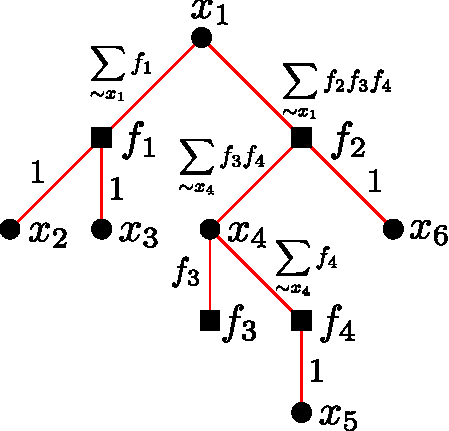
\includegraphics[scale=0.6]{factor_graph_step4}
  \end{subfigure}
  \hspace{1.5cm}
  \begin{subfigure}{0.3\textwidth}
    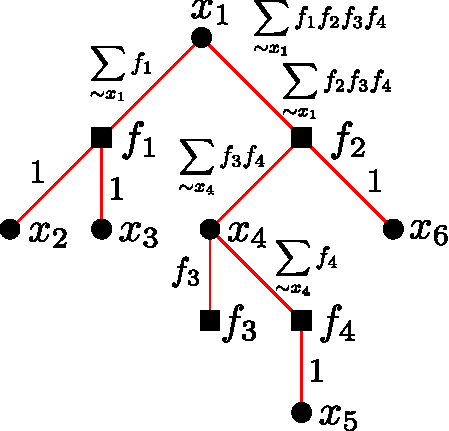
\includegraphics[scale=0.6]{factor_graph_step5}
  \end{subfigure}
   \end{figure}

  \end{frame}
  
  \begin{frame}{Belief Propagation Decoding}
  Bitwise maximum a posteriori (MAP) decoding for memoryless channel without feedback.
  \begin{eqnarray}
  \hat x_i( y) 	&=& \text{arg} \max_{x_i}p_{X_{i}|Y}(x_{i}| y) \label{eq:1}\\
		&=& \text{arg} \max_{x_i}\sum_{\sim x_i}p_{X|Y}( x| y) \label{eq:2}\\
		&=& \text{arg} \max_{x_i}\sum_{\sim x_i}p_{Y|X}( y| x)p_{X}( x) \label{eq:3}\\
		&=& \text{arg} \max_{x_i}\sum_{\sim x_i}\prod_{j}p_{Y_j|X_j}(y_j|x_j)p_{X}( x)\label{eq:4} \\
   		&=& \text{arg} \max_{x_i}\sum_{\sim x_i}\prod_{j}p_{Y_j|X_j}(y_j|x_j)\mathbf{1}_{\left\lbrace x\in C\right\rbrace} \label{eq:5}
  \end{eqnarray} 
  \end{frame}


  \begin{frame}{An Example}
   Given the parity check matrix
\begin{equation}
\label{H_matrix}
 \textbf{H} = 
 \left(
\begin{array}{ccccccc}
1 & 0 & 0 & 1 & 0 & 1 & 1  \\
0 & 1 & 0 & 1 & 1 & 1 & 0  \\
0 & 0 & 1 & 0 & 1 & 1 & 1 
\end{array}
\right)
\end{equation}
\fontsize{7pt}{7.2}\selectfont
\begin{equation}
\hat x_i(y) = \text{arg} \max_{x_i}\sum_{\sim x_i}\prod_{j}p_{Y_j|X_j}(y_j|x_j)\mathbf{1}_{\left\lbrace x_1 + x_4 + x_6 + x_7 = 0\right\rbrace}\mathbf{1}_{\left\lbrace x_2 + x_4 + x_5 + x_6 = 0\right\rbrace}\mathbf{1}_{\left\lbrace x_3 + x_5 + x_6 + x_7 = 0\right\rbrace} \label{eq:decoding_example}
\end{equation}
\begin{figure}[scale=0.5, !tp]
  \centering
  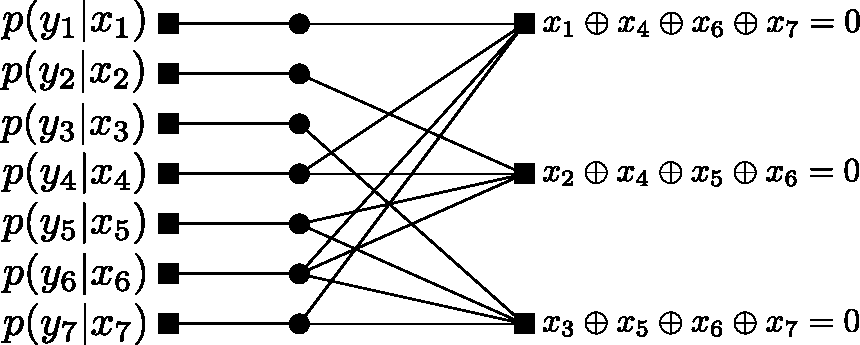
\includegraphics[scale=0.5]{factor_graph_channel}
\end{figure}
  \end{frame}
  
  \begin{frame}{Message Passing Rules - Simplifications}
  \begin{itemize} \itemsep 0.2cm
  \item In the binary case the message is $\left( \mu(1), \mu(-1)\right)$.
  \item $\left( \mu(1), \mu(-1)\right) \gets \left( p_{y_i|x_i}(y_i|1), p_{y_i|x_i}(y_i|-1)\right)$
  \item At a variable node of degree $K + 1$,
  \begin{equation*}
    \mu(1) = \prod_{k = 1}^K \mu_k(1), \quad \mu(-1) = \prod_{k = 1}^K \mu_k(-1)
    \end{equation*}
  \item $r_k \gets \mu_k(1)/\mu_k(-1)$
  \begin{equation*}
   r = \dfrac{\mu(1)}{\mu(-1)} = \dfrac{\prod_{k = 1}^K \mu_k(1)}{\prod_{k = 1}^K \mu_k(-1)} = \prod_k r_k
  \end{equation*}
  \item If $l_k = \log(r_k)$, processing rule becomes $l = \sum_k l_k$

  \end{itemize}
  \end{frame}
  
 \begin{frame}{Message Passing Rules - Simplifications}
 \begin{itemize} \itemsep 0.2cm
  \item At a check node of degree $J + 1$ the computation is
  \begin{equation}
   \mu(x) = \sum_{x_1, x_2, \cdots, x_J} \mathbf{1}_{\lbrace \prod_{j = 1}^J x_j = x\rbrace} \prod_{j = 1}^J \mu_j(x_j)
  \end{equation}
  \begin{eqnarray}
   r = \dfrac{\mu(1)}{\mu(-1)} &=& \dfrac{\sum_{\lbrace x_1, x_2, \cdots, x_J : \prod_{j = 1}^J x_j = 1\rbrace} \prod_{j = 1}^J \mu_j(x_j)}{\sum_{\lbrace x_1, x_2, \cdots, x_J : \prod_{j = 1}^J x_j = -1 \rbrace} \prod_{j = 1}^J \mu_j(x_j)} \\
   &=& \dfrac{\sum_{\lbrace x_1, x_2, \cdots, x_J : \prod_{j = 1}^J x_j = 1\rbrace} \prod_{j = 1}^J \dfrac{\mu_j(x_j)}{\mu_j(-1)}}{\sum_{\lbrace x_1, x_2, \cdots, x_J : \prod_{j = 1}^J x_j = -1\rbrace} \prod_{j = 1}^J \dfrac{\mu_j(x_j)}{\mu_j(-1)}}
  \end{eqnarray}

 
 \end{itemize}
 
 \end{frame}
 \begin{frame}{Message Passing Rules - Simplifications}
    \begin{eqnarray}
   r &=& \dfrac{\sum_{\lbrace x_1, x_2, \cdots, x_J : \prod_{j = 1}^J x_j = 1 \rbrace} \prod_{j = 1}^J r_j^{(1 + x_j)/2}}{\sum_{\lbrace x_1, x_2, \cdots, x_J : \prod_{j = 1}^J x_j = -1\rbrace} \prod_{j = 1}^J r_j^{(1 + x_j)/2}} \\
   &=& \dfrac{\prod_{j = 1}^J (r_j + 1) + \prod_{j = 1}^J (r_j - 1)}{\prod_{j = 1}^J (r_j + 1) - \prod_{j = 1}^J (r_j - 1)} \\
   &=& \dfrac{1 + \dfrac{\prod_{j = 1}^J (r_j - 1)}{\prod_{j = 1}^J (r_j + 1)}}{1 - \dfrac{\prod_{j = 1}^J (r_j - 1)}{\prod_{j = 1}^J (r_j + 1)}} \\
   \implies \dfrac{r - 1}{r + 1} &=& \prod_{j = 1}^{J} \dfrac{r_j - 1}{r_j + 1}
  \end{eqnarray}
 \end{frame}

 \begin{frame}{Message Passing Rules - Simplifications}
  \begin{eqnarray}
   r &=& \exp (l) \\
   \implies \tanh(l/2) &=& \dfrac{r - 1}{r + 1} \\
   &=& \prod_{j = 1}^{J} \dfrac{r_j - 1}{r_j + 1} \\
   &=& \prod_{j = 1}^{J} \tanh(l_j/2) \\
   \implies l &=& 2\tanh^{-1} \left( \prod_{j = 1}^{J} \tanh(l_j/2) \right)
  \end{eqnarray}
 \end{frame}
 
 \begin{frame}{Construction of Parity Check Matrices}
  \begin{itemize}\itemsep 0.3cm
   \item Ideally we need tree.
   \item In practice we try to achieve a minimum girth in the tanner graph.
   \item Construction of Parity Check matrix from Reed Solomon codes.
   \begin{itemize}
    \item Minimum girth of 4 is guaranteed.
    \item Constructs a regular LDPC code.
   \end{itemize}
   \item Progressive Edge Growth construction
   \begin{itemize}
    \item Starts with a graph with no edges.
    \item Progressively introduce edges such that it has minimum effect on the girth
    \item Outputs both regular and irregular LDPC codes.
   \end{itemize}
  \end{itemize}
 \end{frame}
 
   \begin{frame}{Encoding}
   If the parity check matrix is given as $\mathbf{\left[{I \; P}\right]}$, where $\mathbf{I}$ is $N - K$ x $N - K$ identity matrix, $\mathbf{P}$ is some $N - K$ x $K$ matrix,
   a codeword $\mathbf{x = \left[x_p^{\mathsf{T}} \; x_d^{\mathsf{T}}\right]^{\mathsf{T}}}$ can be formed by assigning
    \begin{equation}\nonumber
    \mathbf{x_p = P \cdot x_d}
    \end{equation}
   We obtain $\mathbf{G = \left[{I \; P}\right]}$ from $\mathbf{H}$ by
   \begin{itemize}
    \item Column permutation
    \item Row additions
    \item Row permutations
   \end{itemize}
   Suppose $f$ represents the permutation in obtaining $\mathbf{G}$ from $\mathbf{H}$, and $\mathbf{G \cdot x = 0}$, then $\mathbf{H} \cdot f(\mathbf{x}) = \mathbf{0}$  
  \end{frame}

  \begin{frame}{Belief Propagation Decoding for 2 User Gaussian MAC}
    \begin{eqnarray}
  \hat{x}_i^{[1]} 	&\overset{\Delta}{=}& \text{arg} \max_{x_i}p_{X_i^{[1]}|Y}(x_i^{[1]}|y) \label{eq:mac1} \\
 			&=& \text{arg} \max_{x_i}\sum_{\sim x_i^{[1]}} p_{X^{[1]}, X^{[2]}|Y} (x^{[1]}, x^{[2]}|y)  \label{eq:mac2}\\
 			&=& \text{arg} \max_{x_i}\sum_{\sim x_i^{[1]}} p_{Y|X^{[1]}, X^{[2]}} (y|x^{[1]}, x^{[2]}) p_{X^{[1]}, X^{[2]}}(x^{[1]}, x^{[2]}) \label{eq:mac3}\\
 			&=& \text{arg} \max_{x_i}\sum_{\sim x_i^{[1]}} p_{Y|X^{[1]}, X^{[2]}} (y|x^{[1]}, x^{[2]}) p_{X^{[1]}}(x^{[1]}) p_{X^{[2]}}(x^{[2]}) \label{eq:mac4}\\
 			&=& \text{arg} \max_{x_i}\sum_{\sim x_i^{[1]}} \prod_j p_{Y_j|X_j^{[1]}, X_j^{[2]}} (y_j|x_j^{[1]}, x_j^{[2]}) \mathbf{1}_{\lbrace x^{[1]} \in \mathcal{C}^{[1]}\rbrace} \mathbf{1}_{\lbrace x^{[2]} \in \mathcal{C}^{[2]}\rbrace} \label{eq:mac5}
 \end{eqnarray}
  \end{frame}

  \begin{frame}{Factor Graph for Joint Decoding}
   \begin{figure}
 \centering
 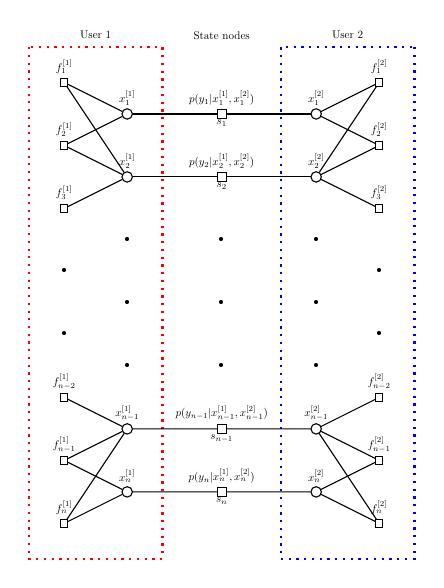
\begin{tikzpicture}[scale=0.4, every node/.style={scale=0.4}]
   \tikzstyle{snode}=[rectangle, draw, inner sep=4pt]
   \tikzstyle{cnode}=[rectangle, draw]
   \tikzstyle{vnode}=[circle, draw]
   
   % Writing comments
   \draw (0, 2.5) node{State nodes};
   \draw (-4, 2.5) node{User 1};
   \draw (4, 2.5) node{User 2};
   % state nodes
   \draw (0, 0) node[snode] (s1) {};
   \draw (0, 0.5) node {$p(y_1|x_1^{[1]}, x_1^{[2]})$};
   \draw (0, -0.3) node {$s_1$};
   \draw (0, -2) node[snode] (s2) {};
   \draw (0, -1.5) node{$p(y_2|x_2^{[1]}, x_2^{[2]})$};
   \draw (0, -2.3) node {$s_2$};
   \draw (0, -4) node{\textbullet};
   \draw (0, -6) node{\textbullet};
   \draw (0, -8) node{\textbullet};
   \draw (0, -10) node[snode] (sn1) {};
   \draw (0, -9.5) node{$p(y_{n-1}|x_{n-1}^{[1]}, x_{n-1}^{[2]})$};
   \draw (0, -10.3) node {$s_{n-1}$};
   \draw (0, -12) node[snode] (sn) {};
   \draw (0, -11.5) node{$p(y_n|x_n^{[1]}, x_n^{[2]})$};
   \draw (0, -12.3) node {$s_n$};
   % User 1 variable nodes
   \draw (-3, 0) node[vnode] (v11) {};
   \draw (-3, 0.5) node {$x_1^{[1]}$};
   \draw (-3, -2) node[vnode] (v12) {};
   \draw (-3, -1.5) node{$x_2^{[1]}$};
   \draw (-3, -4) node{\textbullet};
   \draw (-3, -6) node{\textbullet};
   \draw (-3, -8) node{\textbullet};
   \draw (-3, -10) node[vnode] (v1n1) {};
   \draw (-3, -9.5) node{$x_{n-1}^{[1]}$};
   \draw (-3, -12) node[vnode] (v1n) {};
   \draw (-3, -11.5) node{$x_n^{[1]}$};
   % User 2 variable nodes
   \draw (3, 0) node[vnode] (v21) {};
   \draw (3, 0.5) node {$x_1^{[2]}$};
   \draw (3, -2) node[vnode] (v22) {};
   \draw (3, -1.5) node{$x_2^{[2]}$};
   \draw (3, -4) node{\textbullet};
   \draw (3, -6) node{\textbullet};
   \draw (3, -8) node{\textbullet};
   \draw (3, -10) node[vnode] (v2n1) {};
   \draw (3, -9.5) node{$x_{n-1}^{[2]}$};
   \draw (3, -12) node[vnode] (v2n) {};
   \draw (3, -11.5) node{$x_n^{[2]}$};
   % User 1 check nodes
   \draw (-5, 1) node[cnode] (c11) {};
   \draw (-5, 1.5) node{$f_1^{[1]}$};
   \draw (-5, -1) node[cnode] (c12) {};
   \draw (-5, -0.5) node{$f_2^{[1]}$};
   \draw (-5, -3) node[cnode] (c13) {};
   \draw (-5, -2.5) node{$f_3^{[1]}$};
   \draw (-5, -5) node{\textbullet};
   \draw (-5, -7) node{\textbullet};
   \draw (-5, -9) node[cnode] (c1n2) {};
   \draw (-5, -8.5) node{$f_{n-2}^{[1]}$};
   \draw (-5, -11) node[cnode] (c1n1) {};
   \draw (-5, -10.5) node{$f_{n-1}^{[1]}$};
   \draw (-5, -13) node[cnode] (c1n) {};
   \draw (-5, -12.5) node{$f_n^{[1]}$};
   % User 2 check nodes
   \draw (5, 1) node[cnode] (c21) {};
   \draw (5, 1.5) node{$f_1^{[2]}$};
   \draw (5, -1) node[cnode] (c22) {};
   \draw (5, -0.5) node{$f_2^{[2]}$};
   \draw (5, -3) node[cnode] (c23) {};
   \draw (5, -2.5) node{$f_3^{[2]}$};
   \draw (5, -5) node{\textbullet};
   \draw (5, -7) node{\textbullet};
   \draw (5, -9) node[cnode] (c2n2) {};
   \draw (5, -8.5) node{$f_{n-2}^{[2]}$};
   \draw (5, -11) node[cnode] (c2n1) {};
   \draw (5, -10.5) node{$f_{n-1}^{[2]}$};
   \draw (5, -13) node[cnode] (c2n) {};
   \draw (5, -12.5) node{$f_n^{[2]}$};
   
   % Boxing
   \draw[red,thick,dotted] ($(c11.north west)+(-1,1)$)  rectangle ($(v1n.south east)+(1,-2)$);
   \draw[blue,thick,dotted] ($(c21.north east)+(1,1)$)  rectangle ($(v2n.south west)+(-1,-2)$);
   
   % State user 1 path
   \draw (v11) -- (s1);
   \draw (v12) -- (s2);
   \draw (v1n1) -- (sn1);
   \draw (v1n) -- (sn);
   % State user 2 path
   \draw (v21) -- (s1);
   \draw (v22) -- (s2);
   \draw (v2n1) -- (sn1);
   \draw (v2n) -- (sn);
   
   %user 1 upper connections
   \draw (v11) -- (c11);
   \draw (v12) -- (c11);
   \draw (v11) -- (c12);
   \draw (v12) -- (c13);
   \draw (v12) -- (c12);
   %user 1 lower connections
   \draw (v1n) -- (c1n);
   \draw (v1n1) -- (c1n);
   \draw (v1n) -- (c1n1);
   \draw (v1n1) -- (c1n2);
   \draw (v1n1) -- (c1n1);
   %user 2 upper connections
   \draw (v21) -- (c21);
   \draw (v22) -- (c21);
   \draw (v21) -- (c22);
   \draw (v22) -- (c23);
   \draw (v22) -- (c22);
   %user 2 lower connections
   \draw (v2n) -- (c2n);
   \draw (v2n1) -- (c2n);
   \draw (v2n) -- (c2n1);
   \draw (v2n1) -- (c2n2);
   \draw (v2n1) -- (c2n1);
 \end{tikzpicture}
\end{figure}
  \end{frame}

  \begin{frame}{Message Passing Rules for Joint Decoding}
   \begin{itemize}\itemsep 0.4cm
    \item At variable nodes and at Check nodes the rules are the same.
    \item Rule for the function node
    \fontsize{7pt}{7.2}\selectfont
    \begin{eqnarray}
  \mu_{s_i \rightarrow x_i^{[2]}} &=& \log \left( \dfrac{\exp( \mu_{x_i^{[1]} \rightarrow s_i}) p(y|x_i^{[1]} = -1, x_i^{[2]} = -1) + p(y|x_i^{[1]} = 1, x_i^{[2]} = -1)}{\exp( \mu_{x_i^{[1]} \rightarrow s_i}) p(y|x_i^{[1]} = -1, x_i^{[2]} = 1) + p(y|x_i^{[1]} = 1, x_i^{[2]} = 1)} \right) \\
  \mu_{s_i \rightarrow x_i^{[1]}} &=& \log \left( \dfrac{\exp( \mu_{x_i^{[2]} \rightarrow s_i}) p(y|x_i^{[1]} = -1, x_i^{[2]} = -1) + p(y|x_i^{[1]} = -1, x_i^{[2]} = 1)}{\exp( \mu_{x_i^{[2]} \rightarrow s_i}) p(y|x_i^{[1]} = 1, x_i^{[2]} = -1) + p(y|x_i^{[1]} = 1, x_i^{[2]} = 1)} \right)
  \end{eqnarray}
   \end{itemize}
  \end{frame}

     \begin{frame}{Results - Bit Error Rate Performance}
  (3, 6) Regular Code of block length $N = 96$, dimension $K = 50$, \\
  Number of parity checks $M = 48$,  $10^7$ Bytes Transferred
\begin{center}
 \begin{tabular}{| l | l | l | l | l |}
 \hline
 {}	&  \multicolumn{2}{c|}{No Code} 	&  \multicolumn{2}{c|}{With LDPC}		\\ \hline
  sigma & Errors		& BER		& Errors		& BER		 	\\ \hline
  0.3  	& 4338			& 0.0004338	& 0			& 0			\\ \hline
  0.4	& 61814			& 0.0061814	& 0			& 0			\\ \hline
  0.5	& 227228		& 0.0227228	& 31			& 3.1e-06		\\ \hline
  0.6	& 477744		& 0.0477744	& 65855			& 0.0065855		\\ \hline
  0.7	& 765326		& 0.0765326	& 572393		& 0.0572393		\\ \hline
  0.8	& 1055848		& 0.1055848	& 968856		& 0.0968856		\\ \hline
  0.9	& 1332039		& 0.1332039	& 1291208		& 0.1291208		\\ \hline
  1.0	& 1585653		& 0.1585653	& 1565803		& 0.1565803		\\ \hline
 \end{tabular}
\end{center}
\end{frame}

\begin{frame} {Results - Block Error Rate Performance}
LDPC generated using PEG Algorithm, \\ 
Block length $N = 1008$, Dimension $K = 504$ \\
Number of Parity Checks $M = 504$
\begin{center}
 \begin{tabular}{| c | c | c | c | c |}
 \hline
 {}	&  \multicolumn{2}{c|}{No Code} 	&  \multicolumn{2}{c|}{With LDPC}		\\ \hline
  sigma & Errors		& BER		& Errors		& BER		 	\\ \hline
  0.3  	& 3898			& 0.196461	& 0			& 0			\\ \hline
  0.4	& 18938			& 0.954488	& 0			& 0			\\ \hline
  0.5	& 19840			& 0.999994	& 0			& 0			\\ \hline
  0.6	& 19841			& 1.0		& 17			& 0.0008568		\\ \hline
  0.7	& 19841			& 1.0		& 19841			& 1.0			\\ \hline
 \end{tabular}
\end{center}
\end{frame}

\begin{frame}{Results - Plots}
 \begin{figure}
  \centering
  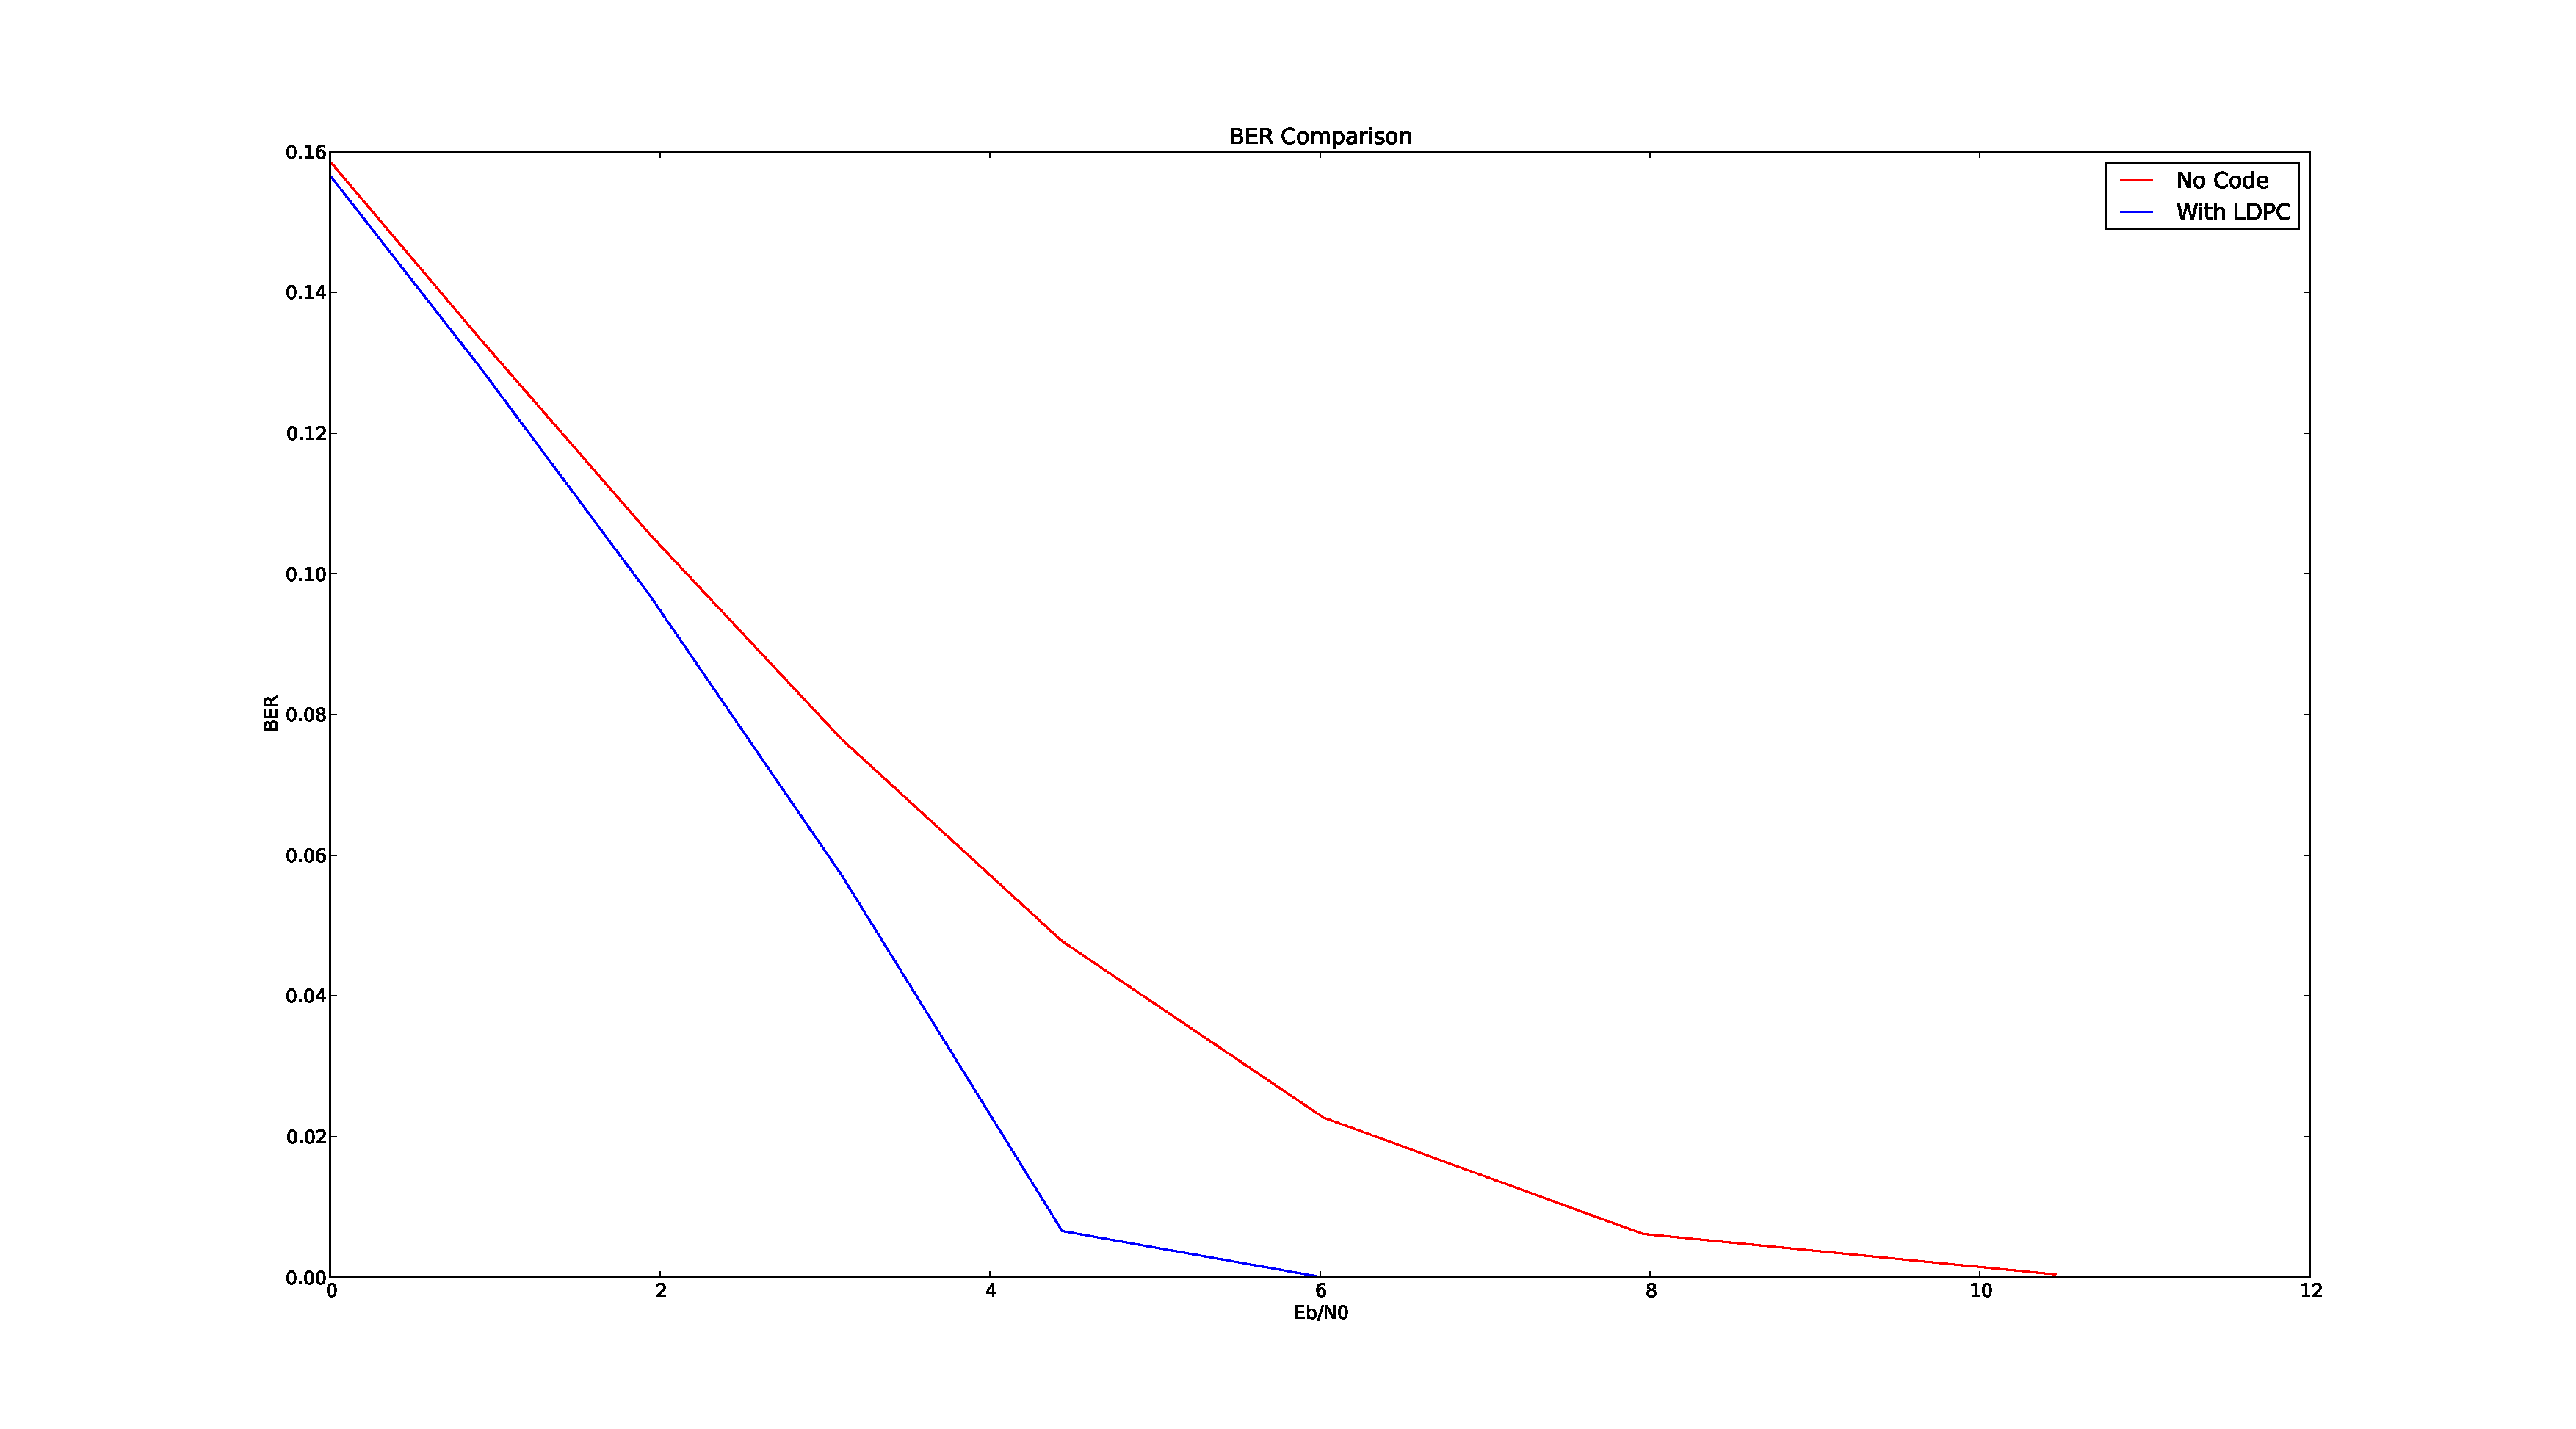
\includegraphics[scale=0.5]{ber_plot}
\end{figure}
\end{frame}

\begin{frame}{gr-ldpc module in GNU Radio}
  \begin{figure}
  \centering
  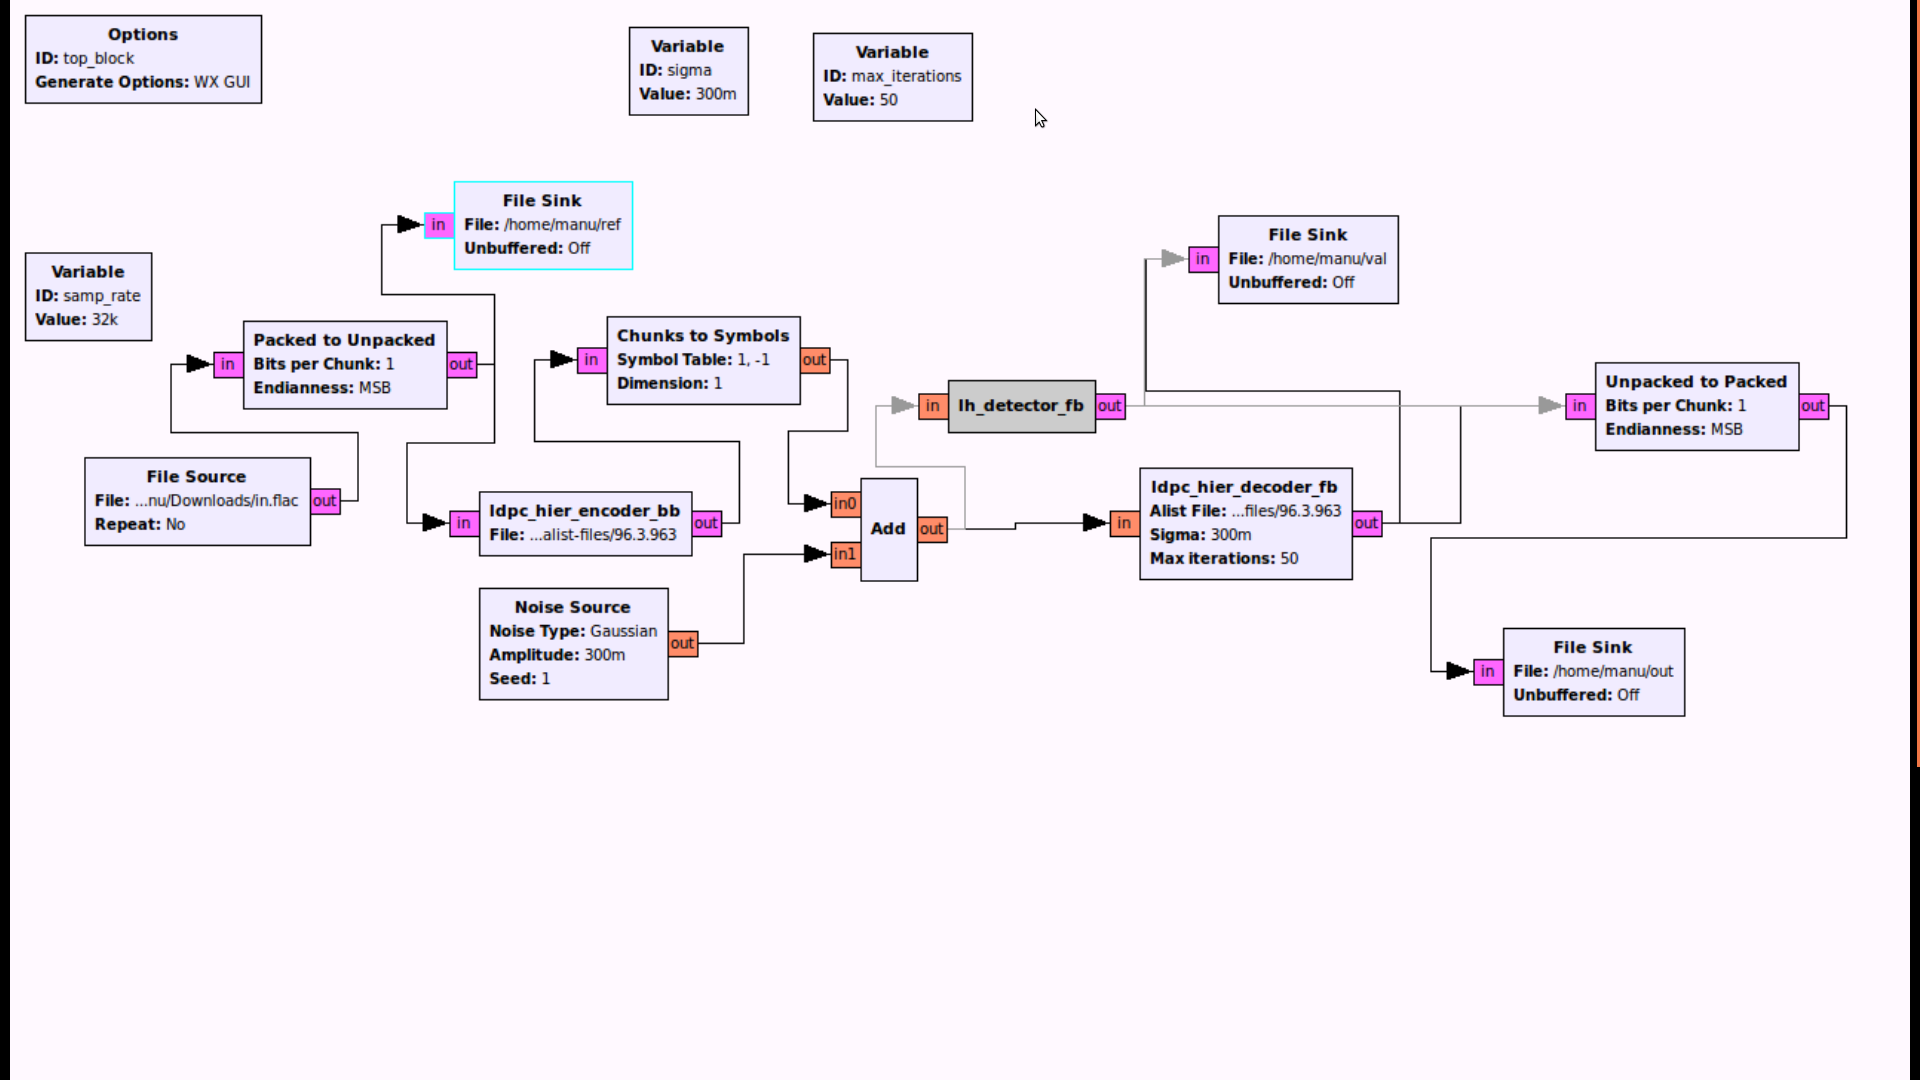
\includegraphics[scale=0.17]{ldpc}
\end{figure}
\end{frame}

\begin{frame}{Rate - Capacity comparison}
 \begin{figure}
 \centering
  \begin{tikzpicture}
  \path [draw, thick, -latex] (0, 0) -- node[at end, left]{$R^{[2]}$} (0, 5) ;
  \path [draw, thick, -latex] (0, 0) -- node[at end, above]{$R^{[1]}$} (5, 0) ;
  \path [draw, latex] (0, 3.4827) -- (1.272, 3.4827);
  \path [draw, latex] (1.272, 3.4827) -- (3.4827, 1.272);
  \path [draw, latex] (3.4827, 1.272) -- (3.4827, 0);
  \draw [dotted, thick] (1.272, 3.4827) -- (1.272, 0);
  \draw [dotted, thick] (3.4827, 1.272) -- (0, 1.272);
  \draw (2, 4) node (val) {$(0.4240, 1.1609)$};
  \path [draw, -latex] (val) -- (1.272, 3.4827);
  \draw (1.5, 1.5) node (bull) {\textbullet};
  \draw (3, 3) node (pair) {$(0.5, 0.5)$};
  \draw (5, 5) node {$\sigma = 0.5$};
  \path [draw, -latex] (pair) -- (1.54, 1.54);
  \end{tikzpicture}
\end{figure}
For single user at $\sigma = 0.8$ (capacity = 0.678) all blocks were decoded correctly.
\end{frame}

\begin{frame}{Future Work}
 \begin{itemize} \itemsep 0.3cm
 \item Study of Density Evolution and EXIT Charts.
  \item 2 users with sample offset of 0.5 symbol duration.
  \item Encoder using sparse LU decomposition
  \item Using VOLK
 \end{itemize}

\end{frame}

\end{document}
